
\begin{figure}[h!]
    \centering
    \caption{Share of low-income residents and workers in the Chicago-Naperville-Elgin CBSA, 2018}
    \label{fig:map_shares_chicago_2018}

    \begin{subfigure}{.5\textwidth}
        \caption{Residents}
        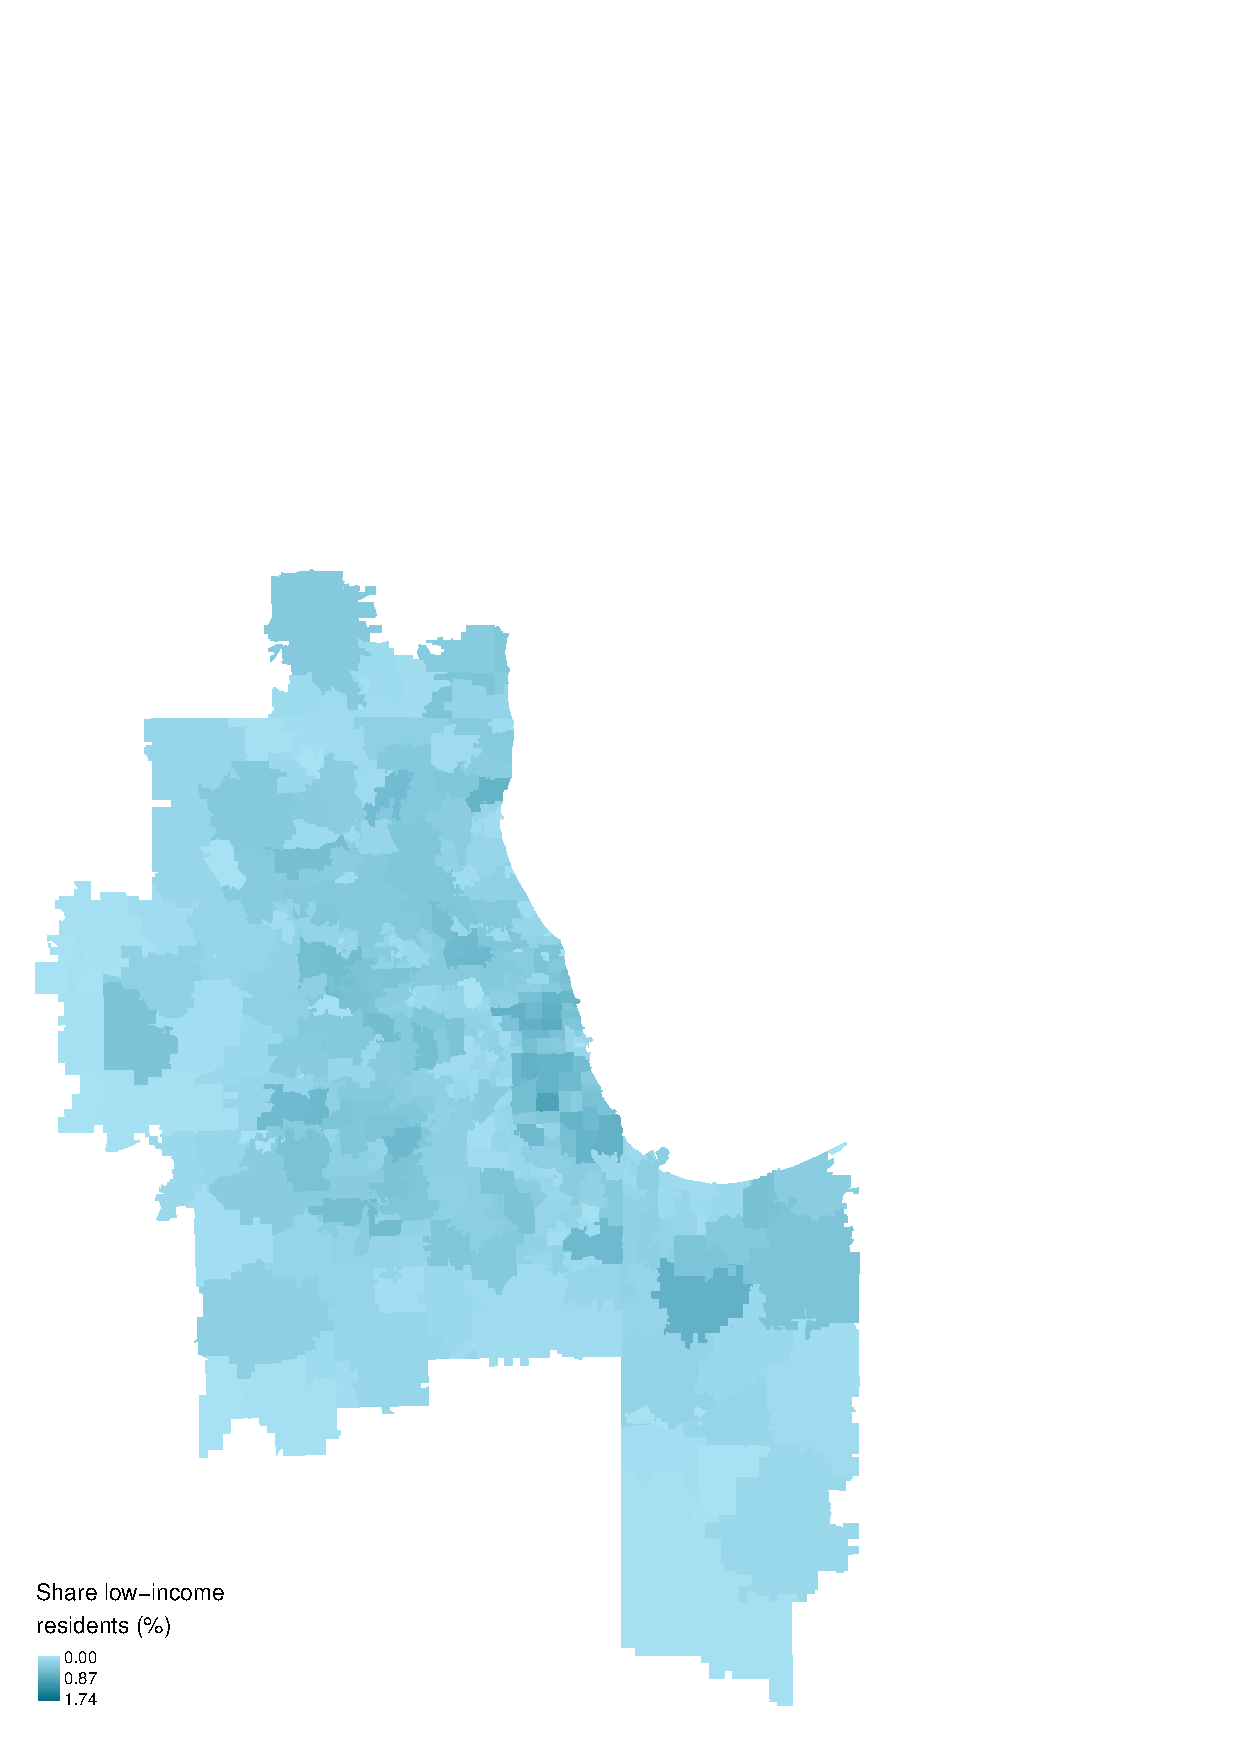
\includegraphics[width = 1\textwidth]
            {maps_shares/output/chicago2018_share_residents_lowinc}
    \end{subfigure}%
    \begin{subfigure}{.5\textwidth}
        \caption{Workers}
        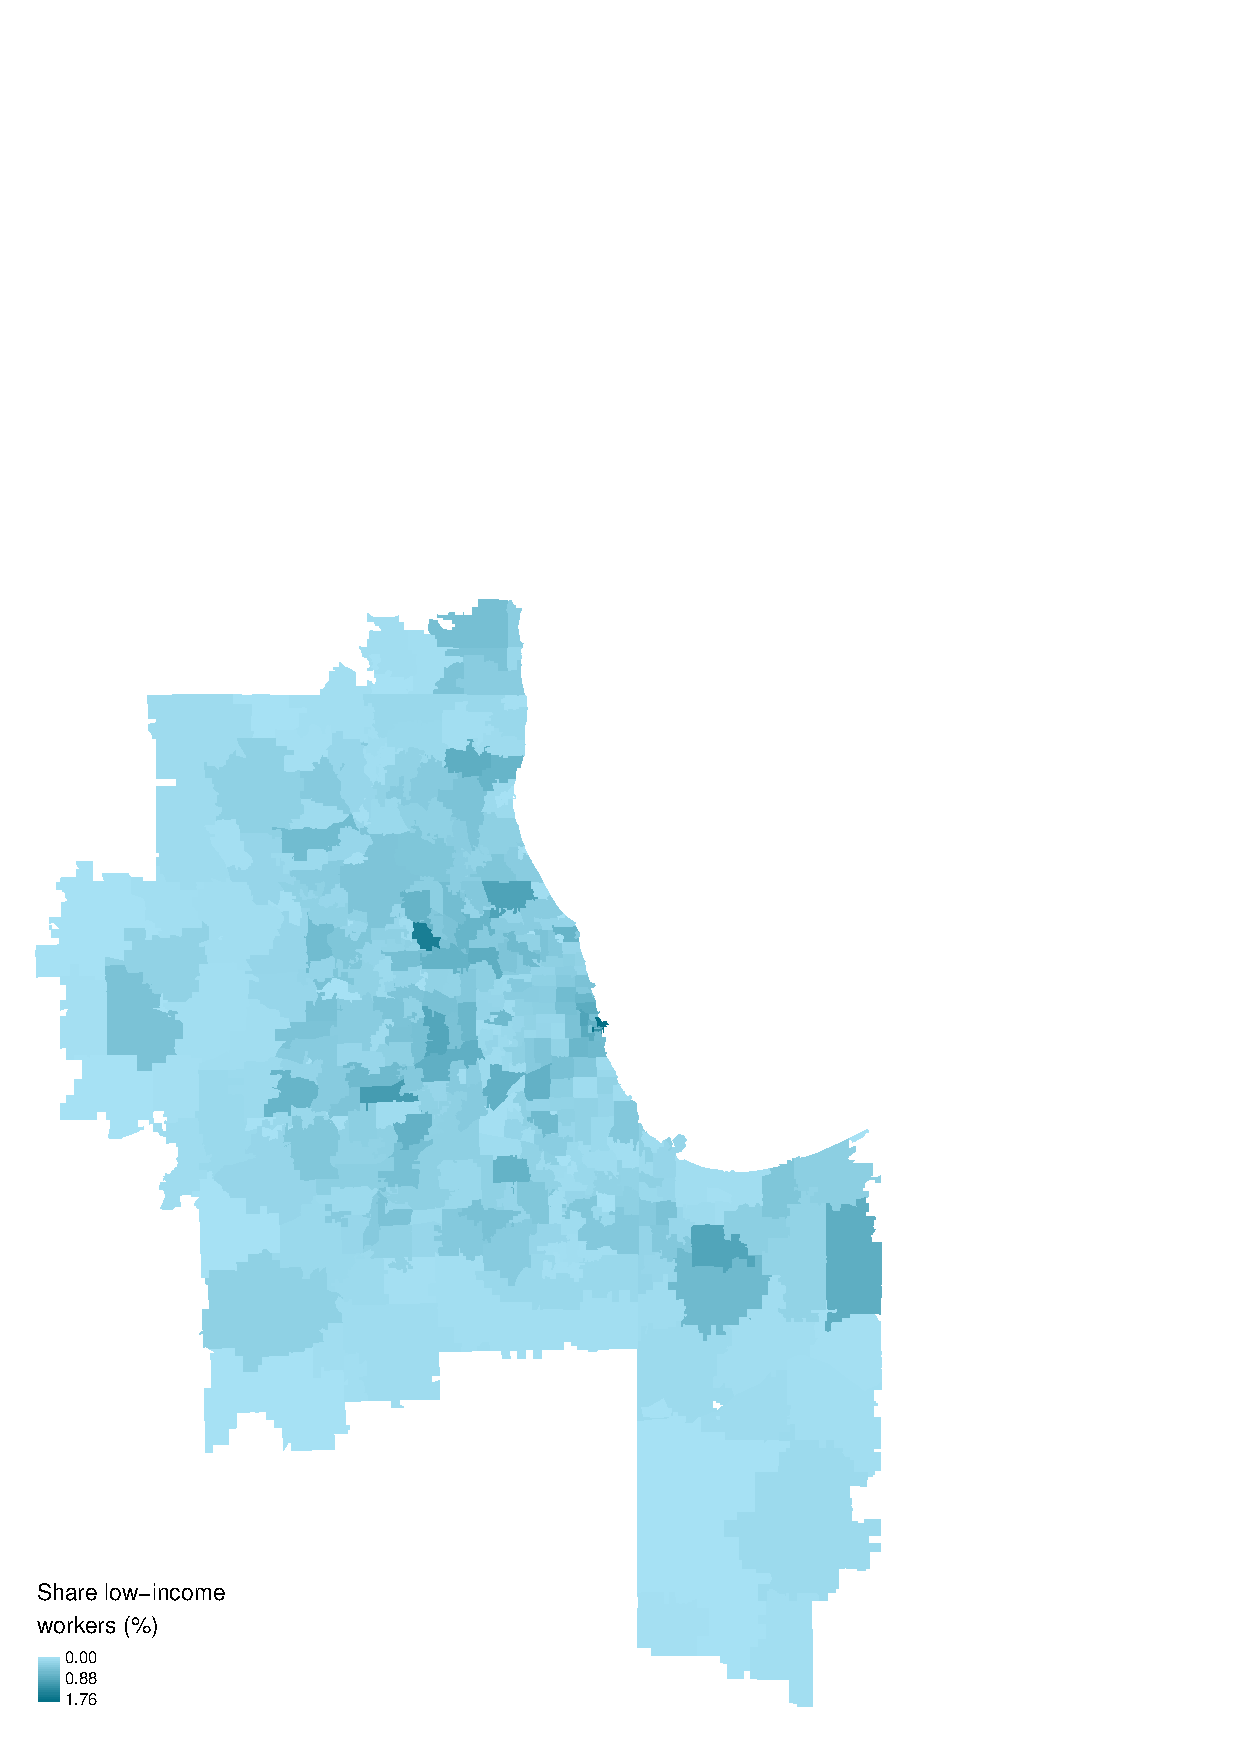
\includegraphics[width = 1\textwidth]
            {maps_shares/output/chicago2018_share_workers_lowinc}
    \end{subfigure}

    \begin{minipage}{.95\textwidth} \footnotesize
        \vspace{3mm}
        Notes:
        Data are from LODES \parencite{CensusLODES} aggregated at the ZIP code level
        using the procedure described in Section \ref{sec:mw_construction}.
        The figure shows the share of low-income residents and workers out of
        the CBSA total in each ZIP code.
        Low-income workers are defined as those earning less than \$1,251 per
        month.
    \end{minipage}
\end{figure}
